% ArtPoW whitepaper. Build: `pdflatex whitepaper.tex` (twice), `latexmk -pdf whitepaper.tex` or `tectonic whitepaper.tex`.
\documentclass[10pt,letterpaper]{article}

\usepackage[T1]{fontenc}
\usepackage[utf8]{inputenc}
\usepackage{mathptmx}
\usepackage[letterpaper,top=1in,bottom=1in,left=1.15in,right=1.15in]{geometry}
\usepackage{amsmath}
\usepackage{booktabs}
\usepackage{tikz}
\usetikzlibrary{arrows.meta,positioning,calc}
\usepackage{titlesec}
\usepackage{parskip}
\usepackage{enumitem}
\usepackage{microtype}
\usepackage{caption}
\usepackage[hidelinks]{hyperref}

% Section headings in the style of the Bitcoin paper: "1. Introduction", bold, no extra decoration.
\titleformat{\section}{\normalfont\bfseries\large}{\thesection.}{0.5em}{}
\titlespacing*{\section}{0pt}{14pt}{4pt}
\titleformat{\subsection}{\normalfont\bfseries}{\thesubsection}{0.5em}{}
\titlespacing*{\subsection}{0pt}{8pt}{2pt}
\setlist{nosep,leftmargin=1.6em}
\renewcommand{\arraystretch}{1.15}

\newcommand{\fn}[1]{\texttt{#1}}

\begin{document}

\begin{center}
  {\Large\bfseries ArtPoW: A Free Monthly NFT Earned by Proof of Work}\\[10pt]
  theophilewalter.eth\\
  % Add the project website here once it exists.
\end{center}

\vspace{4pt}
\begin{list}{}{\leftmargin=0.45in\rightmargin=0.45in}\item\relax
\textbf{Abstract.} We describe a collection of non-fungible tokens on Polygon in which a new edition, created by a
guest artist, opens every month and can be claimed for free by anyone, directly on-chain or through a website. A
claim requires a proof of work tied to its recipient, so it cannot be stolen and anyone may submit it. The
difficulty follows a linear schedule of one thousand tokens per month: every token minted ahead of the schedule
makes the next one harder, while time eases it back to a floor of about one minute of browser mining. There is no
cap on the number of tokens; supply regulates itself, and an attacker's excess grows only with the logarithm of
its computing power. The seed of each month is an accumulator of every claim of the previous month, so the
puzzle of a month is unknown until the previous month ends. Metadata are generated on-chain, the contract cannot
be upgraded, its parameters are constants, and no royalty is charged.
\end{list}

\section{Introduction}

Free distributions of digital collectibles usually face two problems. Without a cost, automated accounts claim
most of the supply; with a price or an allow-list, the distribution is no longer open. Proof of work, introduced
as an anti-abuse measure by Hashcash~[9] and used by Bitcoin to order transactions~[1], gives a third option: a
claim costs a measurable amount of computation, which anyone can provide and anyone can verify.

This paper describes ArtPoW, an ERC-721 contract~[3] that applies this idea to a monthly edition. Each month, a guest artist creates
the artwork; any address can claim one token by mining a nonce in a browser, from the command line or with any
other software. The contract keeps the average issuance close to one thousand tokens per month without a hard
cap, by adjusting the difficulty after every claim against a linear schedule. The rest of the design aims at
staying simple: one seed mechanism, no transaction to open a month, no grace periods, metadata entirely on-chain,
and administrator powers that never extend to the holders' tokens.

Proof of work regulates the supply, not who receives it. A single modern GPU computes as many hashes as about a
thousand browsers; when farms compete, they obtain most of the tokens. Section~\ref{sec:security} quantifies this
and the other limits of the design.

\section{Monthly Editions}

Months are scheduled by administrators, in order and without gaps in their numbering. Each month has a start, an
end and a content: a label (for example ``November 2026''), the artist's name, an optional address receiving the
artist proof, the URI of an artwork and an optional animation URI. The contract enforces that a month:
\begin{itemize}
  \item lasts between 25 and 35 days, which covers calendar months and rejects typing errors that would become
        final once the month starts;
  \item starts in the future and not before the end of the previous month, so months never overlap;
  \item has a non-empty label and image;
  \item can be edited until it starts, and is then locked, dates and content included.
\end{itemize}

A month ends at its scheduled time whatever happens. Claims are accepted while
$\mathit{start} \le \mathit{now} < \mathit{end}$; if the next month is not scheduled yet, no claim is possible
until it starts. Months are expected to be contiguous: the next one starts when the previous one ends.

\section{Proof of Work}

To claim a token of month $m$ for a recipient $r$, one finds a nonce $n$ such that
\[
  H = \mathrm{keccak256}\big(\mathrm{abi.encode}(\mathit{seed}_m,\ m,\ r,\ n)\big) < T ,
\]
where $T$ is the target at the time the claim is included in a block (Section~\ref{sec:difficulty}). The encoded
message is 128 bytes long, a single Keccak-256 block~[8], so every attempt costs exactly one permutation, on a
GPU as in a browser.

The recipient is part of the hash. A proof found for $r$ is useless for any other address: whoever submits it,
the token goes to $r$. Proofs therefore cannot be stolen, and anyone may submit a claim on behalf of anyone else.
Each address can claim at most one mined token per month; transferring the token does not allow a second claim.

A proof is checked against the target at inclusion, not at the time it was found. Time only makes the target
easier; claims included in the meantime make it harder, by about 7\% each. Miners therefore aim at the target the
contract would have after one or two more claims, which costs about 15\% more work and makes stale proofs
negligible in practice.

\section{Seed Chain}

The seed of month 1 is the hash of the block preceding the deployment. Every month keeps an accumulator,
initialised to $\mathrm{keccak256}(\mathit{seed}_m, m)$ and updated by every claim:
\[
  \mathit{acc}_m \leftarrow \mathrm{keccak256}\big(\mathit{acc}_m,\ \mathrm{blockhash}(b-1),\ r,\ n\big),
\]
where $b$ is the block of the claim. The seed of the next month is the final accumulator:
$\mathit{seed}_{m+1} = \mathit{acc}_m$. Since every claim changes the accumulator, the puzzle of month $m+1$ is
unknown until month $m$ ends. A month without any claim keeps its initial accumulator, which is accepted: a month
nobody claims is a month nobody is trying to pre-mine.

\begin{figure}[h]
\centering
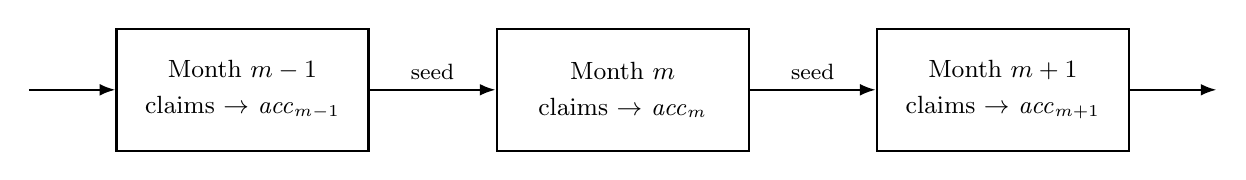
\begin{tikzpicture}[
  month/.style={draw, thick, minimum width=3.2cm, minimum height=1.55cm, align=center, font=\small},
  arr/.style={-{Latex[length=2mm]}, thick}, font=\small]
  \node[month] (a) {Month $m-1$\\[2pt]claims $\to$ $\mathit{acc}_{m-1}$};
  \node[month, right=1.6cm of a] (b) {Month $m$\\[2pt]claims $\to$ $\mathit{acc}_{m}$};
  \node[month, right=1.6cm of b] (c) {Month $m+1$\\[2pt]claims $\to$ $\mathit{acc}_{m+1}$};
  \draw[arr] (a) -- node[above, font=\footnotesize] {seed} (b);
  \draw[arr] (b) -- node[above, font=\footnotesize] {seed} (c);
  \draw[arr] ($(a.west)+(-1.1,0)$) -- (a);
  \draw[arr] (c) -- ($(c.east)+(1.1,0)$);
\end{tikzpicture}
\caption*{\small Each month's seed is the accumulator of all the claims of the previous month.}
\end{figure}

Artist and team proofs (Section~\ref{sec:proofs}) do not touch the accumulator, so administrators cannot influence
the next seed by choosing when to mint them.

\section{Difficulty Schedule}\label{sec:difficulty}

Let $k$ be the number of tokens already mined in the month and $S(t)$ the number the schedule expects at time
$t$:
\[
  S(t) = 1000 \cdot \frac{t - \mathit{start}}{\mathit{end} - \mathit{start}} .
\]
The target is
\[
  T(k, t) = \min\!\Big(T_{\max},\ T_{\max} \cdot 2^{\,(S(t) - k)/10}\Big),
  \qquad T_{\max} = 2^{256-28}.
\]
At the floor $T_{\max}$, a valid hash takes $2^{28} \approx 2.7 \times 10^{8}$ attempts on average, about one minute
in a browser. Each token minted ahead of the schedule multiplies the difficulty by $2^{1/10} \approx 1.07$; ten
tokens ahead double it. Time works the other way: with no claim, the difficulty halves every ten scheduled tokens,
about 7.2 hours in a 30-day month. Behind the schedule, the difficulty stays at the floor and the delay can be
caught up within the month: if few people claimed, whoever arrives can take the rest. Every month restarts from
the floor and targets one thousand tokens whatever its length.

\begin{figure}[h]
\centering
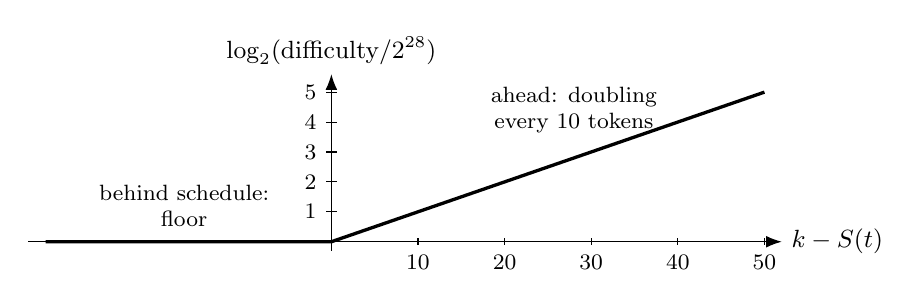
\begin{tikzpicture}[x=0.11cm, y=0.38cm, font=\small]
  \draw[-{Latex[length=2mm]}] (-35,0) -- (52,0) node[right] {$k - S(t)$};
  \draw[-{Latex[length=2mm]}] (0,-0.3) -- (0,5.6) node[above] {$\log_2(\text{difficulty}/2^{28})$};
  \draw[very thick] (-33,0) -- (0,0) -- (50,5);
  \foreach \x in {10,20,30,40,50} \draw (\x,0.12) -- (\x,-0.12) node[below, font=\footnotesize] {\x};
  \foreach \y in {1,...,5} \draw (0.6,\y) -- (-0.6,\y) node[left, font=\footnotesize] {\y};
  \node[font=\footnotesize, align=center] at (-17,1.2) {behind schedule:\\floor};
  \node[font=\footnotesize, align=center] at (28,4.4) {ahead: doubling\\every 10 tokens};
\end{tikzpicture}
\caption*{\small Difficulty as a function of the number of tokens ahead of the schedule.}
\end{figure}

The rule is the per-month form of the ASERT algorithm used by Bitcoin Cash~[2], with the claims of the month in
place of blocks. The target changes after every claim: a burst raises the difficulty as it happens, and no window
lets a fast miner claim many tokens at a stale target.

The contract computes $x \cdot 2^{a/b}$ in fixed point with the cubic approximation of
\texttt{aserti3-2d}~[2]: 16-bit fractional exponent, maximum relative error 0.0117\%, monotonic. The
implementation is checked bit for bit against an independent Python port on random vectors, with the production
floor.

\subsection*{Calculations}

A miner with hash rate $R$ that claims continuously reaches the equilibrium where it finds one token per scheduled
interval $I = (\mathit{end} - \mathit{start})/1000$, that is $R I = 2^{28} \cdot 2^{n/10}$. Its lead on the
schedule is therefore
\[
  n = 10 \log_2 \frac{R\, I}{2^{28}} .
\]
For one GPU at $5 \times 10^9$ hashes per second and a 30-day month ($I = 2592$~s), $n \approx 156$; ten GPUs add
only $10 \log_2 10 \approx 33$ tokens. A farm can take most of a month's tokens, but the month's total stays close
to one thousand plus this lead.

A miner can also accumulate work $W$ before a month starts, whenever the seed is known in advance
(Section~\ref{sec:security}), and submit the results at once. The $j$-th token at the start of the month needs a hash
below $T_{\max} 2^{-j/10}$, and $W$ attempts yield on average $W 2^{-28-j/10}$ such hashes, so the burst $K$
satisfies $W 2^{-28-K/10} \approx K$:
\[
  K \approx 10 \left(\log_2 W - 28 - \log_2 K\right).
\]

\section{Artist and Team Proofs}\label{sec:proofs}

Besides mined tokens, each month may have one artist proof, sent to the artist's address, and one team proof, sent
to an address set by the administrators. Proofs are minted without work by \fn{claimReserved}, which anyone may
call during the month; the token always goes to the designated address, so the website or an administrator can
mint them as soon as the month starts. Each proof exists at most once per month.

Proofs stay out of the numbering, the total and the difficulty schedule, and do not touch the seed. They are also
independent of mined claims: the artist and the team may mine a regular token as well. Since anyone can mine a
claim on behalf of any address, this keeps a third party from blocking a proof by mining a regular token for the
artist first.

The collection charges no royalty. Royalties are optional on most marketplaces and would amount to a fee on the
work of artists who do not receive it; the proofs give the artist and the team a place in the collection, alongside
its collectors.

\section{Metadata}

Token metadata are a JSON document generated by the contract and returned by \fn{tokenURI}, with no server. A mined
token is named after its month and number, for example ``November 2026 $\bullet$ \#256'', and shows the final total
once the month is over: ``November 2026 $\bullet$ \#256 / 1035''. Its attributes are the month, the artist, the
edition (\emph{Mined}, \emph{Artist proof} or \emph{Team proof}), the number, the total, the difficulty at which it
was mined and the number of leading zero bits of its hash, a rarity attribute that the miner can improve by
searching longer. Proofs have no number, difficulty or zero bits.

The total is read when the metadata are requested, so closing a month requires no transaction. Since marketplaces
cache metadata, anyone can call \fn{announceMonthTotal} once after the month ends; it emits the EIP-4906 batch update
event~[4] over the month's tokens, which are contiguous because months never overlap.

Collection metadata follow ERC-7572~[5]: \fn{contractURI} returns the name, the description, the logo and the
website, the last two set by administrators. The website also gives every token a link to its own page. The
\fn{owner} function of ERC-173~[6], which marketplaces use to decide who manages the collection page, returns an
address set by the administrators; it grants no right in the contract.

Images are referenced by URI. The recommended practice is an \fn{ipfs://} content identifier pinned by two
independent services, with a permanent copy on Arweave from which the same identifier can be pinned again. Very
small images can be stored on-chain as \fn{data:} URIs, at about 980 gas per byte.

\section{Administration}

The contract has no proxy and cannot be upgraded; its parameters are constants. Administrators form a list, built on
OpenZeppelin's access control~[7], in which any administrator can add or remove others, so that losing one wallet does not lose the contract. Adding an
administrator takes two steps: an administrator calls \fn{proposeAdmin}, then the proposed address calls
\fn{acceptAdmin} itself. Only an address able to send a transaction on this network can become an administrator,
which rules out the zero address, typing errors and multisig wallets deployed on another network. The last
administrator cannot be removed.

Administrators schedule months that have not started, set the team address, the \fn{owner} address, the logo and
the website, and can recover assets sent to the contract by mistake: native tokens sent by forced transfer, ERC-20
tokens and NFTs of other collections. They can never move, burn or freeze holders' tokens, and tokens of this
collection sent to the contract stay there for good.

In case of a flaw, any administrator can call \fn{shutdown}. It is irreversible and immediate: claims, proofs and
scheduling stop for good, the running month is considered closed, and transfers, metadata and recovery keep
working. A single administrator can trigger it on purpose: stopping a contract by mistake or after a theft of keys
is better than leaving one running with a known flaw, or one that a rogue administrator could keep from being
stopped.

\section{Security Considerations}\label{sec:security}

\textbf{Farms.} Proof of work cannot tell a person from a machine. With one GPU equivalent to about a thousand
browsers, a farm keeps the difficulty at a level where a browser would need weeks per token. The design bounds the
supply, not the farms' share; only a proof of personhood could, which is outside the scope of a contract that
anyone can use directly.

\textbf{Pre-mining.} The seed of a month is public before its start in three cases: between the deployment and the
first month, during a gap between two months, and speculatively at the end of a quiet month, when the last claim
may be final. Work accumulated in these windows can be submitted as a burst when the month opens. The schedule
bounds it as computed above:

\begin{center}
\begin{tabular}{lr}
\toprule
Pre-mined work & Burst at the start of the month \\
\midrule
1 GPU for 3 hours & $\approx 108$ tokens \\
1 GPU for 1 week & $\approx 160$ tokens \\
100 GPUs for 1 month & $\approx 242$ tokens \\
\bottomrule
\end{tabular}
\end{center}

This risk is accepted: the first month opens before the project is widely known, and later months are contiguous.
The participant who submits the very last claim of a month, or the validator producing that block, learns the next
seed seconds before others; the schedule throttles any resulting burst in the same way.

\textbf{Front-running.} A pending claim reveals its nonce, but a copy still mints to the intended recipient. A
competitor can only make a pending proof insufficient by mining claims of its own, which is mining.

\textbf{Compromised administrator.} A compromised administrator cannot touch holders' tokens or mint more than two
free tokens per month. It could remove the other administrators, schedule a month with malicious content, which
becomes permanent once the month starts, point the website link of every token to another site, take over the
collection page through \fn{owner}, or stop the contract. Administration is therefore meant to be held by a
multisig wallet, with alerts on the administrative events.

\textbf{Network.} Block timestamps can be shifted by a few seconds, which moves the schedule by a negligible
fraction of a token. Blocks can be reorganised shortly after they are produced; miners should wait for finality
before mining on a new month's seed, and interfaces before displaying token numbers.

\textbf{Implementation.} All state changes of a claim happen before the only external call, the ERC-721
receiver hook, and re-entering claims leave the state consistent. The contract makes no arbitrary call, has no
\fn{delegatecall} or self-destruct, and embeds administrator-provided strings in its JSON only after rejecting
quotes, backslashes and control characters. Unit, fuzz, invariant and differential tests cover the rules described
here, and the compiler version is pinned so that the deployed bytecode can be verified.

\section{Measurements and Simulations}

The reference miner is a Keccak-f permutation written in WebAssembly. It reaches 2~million hashes per second per
thread in the V8 engine on a 2016 desktop processor, 7.5~million on four cores, twenty times faster than a pure
JavaScript implementation. Assuming a median browser at 4~million hashes per second, the floor takes 67~seconds on
average and 46~seconds in median. A GPU computes about $5 \times 10^9$ single-block Keccak-256 hashes per second.

A Monte-Carlo simulation of a 30-day month models people arriving over the month, each mining in a browser with a
log-normal hash rate and giving up after a log-normal patience, and farms mining continuously with unlimited
addresses. Results, averaged over five runs:

\begin{center}
\begin{tabular}{lrrrr}
\toprule
Scenario & Minted & People & Farms & People served \\
\midrule
300 people & 293 & 293 & 0 & 98\% \\
3000 people (28, 30 or 31 days) & 1054 & 1054 & 0 & 35\% \\
Launch: 2000 people in 48 hours & 680 & 680 & 0 & 26\% \\
300 people, a 64-core server & 1101 & 7 & 1094 & 2\% \\
300 people, 1 GPU all month & 1156 & 0 & 1156 & 0\% \\
300 people, 1 GPU from day 25 & 1157 & 240 & 917 & 80\% \\
3000 people, 1 GPU for 2 hours & 1054 & 973 & 81 & 32\% \\
300 people, 10 GPUs all month & 1188 & 0 & 1188 & 0\% \\
\bottomrule
\end{tabular}
\end{center}

When demand is low, everyone is served within minutes. Above one thousand claims a month, the difficulty limits
issuance and patient people get the tokens. Whatever the attackers' power, a month stays between one thousand and
twelve hundred tokens, while farms take most of them.

\section{Costs}

Gas used by complete transactions, measured on the deployed contract:

\begin{center}
\begin{tabular}{lr}
\toprule
Operation & Gas \\
\midrule
Deployment & 4\,570\,000 \\
Schedule a month (IPFS image / image and animation) & 261\,000 / 351\,000 \\
Claim (the first of a month: $+17\,000$) & 189\,000 \\
Artist or team proof & 135\,000 -- 155\,000 \\
Announce a month's total & 54\,000 \\
Transfer & 84\,000 \\
\bottomrule
\end{tabular}
\end{center}

At a gas price of 267~gwei and 0.082~euro per POL, as observed on 31 October 2026, a claim costs about 0.004~euro
and the deployment about 0.10~euro. The claimant always pays the gas of its claim.

\section{Conclusion}

We have described a free monthly NFT in which access is open to anyone able to compute, and issuance regulates
itself without a cap. Proofs of work are bound to their recipients, so they cannot be stolen and can be submitted by
anyone; a chain of accumulators keeps each month's puzzle unknown until the previous month ends; a difficulty that
follows a linear schedule after every claim keeps a month close to one thousand tokens, an attacker's lead growing
only with the logarithm of its power. Metadata live on-chain, administrators cannot touch the holders' tokens, and
the contract can be stopped but never changed. The design does not decide who receives the tokens when machines
compete with people; it only makes the cost of each token explicit and the rules the same for everyone.

\section*{References}

\begin{enumerate}[label={[\arabic*]},leftmargin=2.2em,itemsep=2pt]
  \item S. Nakamoto, ``Bitcoin: A Peer-to-Peer Electronic Cash System,'' 2008.
  \item Bitcoin Cash, ``ASERT Difficulty Adjustment Algorithm (aserti3-2d),'' upgrade specification, November 2020.
  \item W. Entriken, D. Shirley, J. Evans, N. Sachs, ``EIP-721: Non-Fungible Token Standard,'' 2018.
  \item ``EIP-4906: EIP-721 Metadata Update Extension,'' 2022.
  \item ``ERC-7572: Contract-level metadata via \texttt{contractURI()},'' 2023.
  \item ``ERC-173: Contract Ownership Standard,'' 2018.
  \item OpenZeppelin, ``OpenZeppelin Contracts,'' version 5.
  \item G. Bertoni, J. Daemen, M. Peeters, G. Van Assche, ``The Keccak reference,'' 2011.
  \item A. Back, ``Hashcash -- A Denial of Service Counter-Measure,'' 2002.
\end{enumerate}

\end{document}
